%%%%%%%%%%%%%%%%%%%%%%%%%%%%%%%%%%%%%%%%%%%%%%%%%%%%%%%%%%%%%%%%%%%%
%% I, the copyright holder of this work, release this work into the
%% public domain. This applies worldwide. In some countries this may
%% not be legally possible; if so: I grant anyone the right to use
%% this work for any purpose, without any conditions, unless such
%% conditions are required by law.
%%%%%%%%%%%%%%%%%%%%%%%%%%%%%%%%%%%%%%%%%%%%%%%%%%%%%%%%%%%%%%%%%%%%

\documentclass[
  digital, %% This option enables the default options for the
           %% digital version of a document. Replace with `printed`
           %% to enable the default options for the printed version
           %% of a document.
  notable,   %% Causes the coloring of tables. Replace with `notable`
           %% to restore plain tables.
  lof,     %% Prints the List of Figures. Replace with `nolof` to
           %% hide the List of Figures.
  lot,     %% Prints the List of Tables. Replace with `nolot` to
           %% hide the List of Tables.
  %% More options are listed in the user guide at
  %% <http://mirrors.ctan.org/macros/latex/contrib/fithesis/guide/mu/fi.pdf>.
]{fithesis3}
%% The following section sets up the locales used in the thesis.
\usepackage[resetfonts]{cmap} %% We need to load the T2A font encoding
\usepackage[T1,T2A]{fontenc}  %% to use the Cyrillic fonts with Russian texts.
\usepackage[
  main=english, %% By using `czech` or `slovak` as the main locale
                %% instead of `english`, you can typeset the thesis
                %% in either Czech or Slovak, respectively.
  german, russian, czech, slovak %% The additional keys allow
]{babel}        %% foreign texts to be typeset as follows:
%%
%%   \begin{otherlanguage}{german}  ... \end{otherlanguage}
%%   \begin{otherlanguage}{russian} ... \end{otherlanguage}
%%   \begin{otherlanguage}{czech}   ... \end{otherlanguage}
%%   \begin{otherlanguage}{slovak}  ... \end{otherlanguage}
%%
%% For non-Latin scripts, it may be necessary to load additional
%% fonts:
\usepackage{paratype}
\def\textrussian#1{{\usefont{T2A}{PTSerif-TLF}{m}{rm}#1}}
%%
%% The following section sets up the metadata of the thesis.
\thesissetup{
    date          = 2017/06/04, %\the\year/\the\month/\the\day,
    university    = mu,
    faculty       = fi,
    type          = bc,
    author        = Lenka Svetlovská,
    gender        = f,
    advisor       = {RNDr. Andriy Stetsko, Ph.D.},
    title         = {Security and cryptography in GO},
    TeXtitle      = {Security and cryptography in GO},
    keywords      = {keyword1, keyword2, ...},
    TeXkeywords   = {keyword1, keyword2, \ldots},
    bib           = example.bib,
}
\thesislong{abstract}{
    This is the abstract of my thesis, which can

    span multiple paragraphs.
}
\thesislong{thanks}{
    This is the acknowledgement for my thesis, which can

    span multiple paragraphs.
}
\usepackage{makeidx}      %% The `makeidx` package contains
\makeindex                %% helper commands for index typesetting.
%% These additional packages are used within the document:
\usepackage{paralist} %% Compact list environments
\usepackage{amsmath}  %% Mathematics
\usepackage{amsthm}
\usepackage{amsfonts}
\usepackage{url}      %% Hyperlinks
\usepackage{markdown} %% Lightweight Markup

%added usepackages
%\usepackage{rotating} %rotate table?
%\newcommand*{\TitleInParbox}{\parbox[c]{0.3\linewidth}{\Title}}
\usepackage{longtable}
\usepackage{array}
\newcolumntype{P}[1]{>{\centering\arraybackslash}p{#1}}
\usepackage{enumitem}

\begin{document}
\chapter{Introduction}


\chapter{Basic Terms}
In this section, I define the basic terms which are necessary to an understanding of the text 
presented in the following chapters. First I explain the symmetric and asymmetric cryptography, X.509 
certificates, protocols SSL and TLS. Finally, I describe TLS\_PSK, which is indispensable 
for working with ......

\section{Cryptography}
Cryptography is the study of mathematical techniques related to aspects of information
security such as confidentiality, data integrity, entity authentication, and data origin
authentication \cite{menezes1996handbook}. %Together with cryptanalysis, which is engaged in deciphering codes without the secret knowledge key, is the part of science called cryptology.
%\vskip 0.2in
%Already in the nineteenth century, Auguste Kerckhoffs formulated the principle which has been true in cryptography today. Safety of cryptosystem must not depend on the secrecy of the algorithm. It must be publicly known, and security must depend only on the secret key \cite{menezes1996handbook}. 
Today we talk about computer security which consists in the fact that the attacker does not have 
enough computational strength and time to decode the cipher. 
%Discrete logarithm and factorization of large numbers belong to the issues for which there is no effective algorithm today.
%\vskip 0.2in
We can divide cryptography base on the type of keys into three parts. They are symmetric 
cryptography, asymmetric cryptography, and other primitives %, for example, hash functions, one-way permutation or random number generators
\cite{menezes1996handbook}%%, see Figure \ref{fig:secPrim}
.

%%OBRAZOK
%\begin{figure}[th]
%	\centering
%	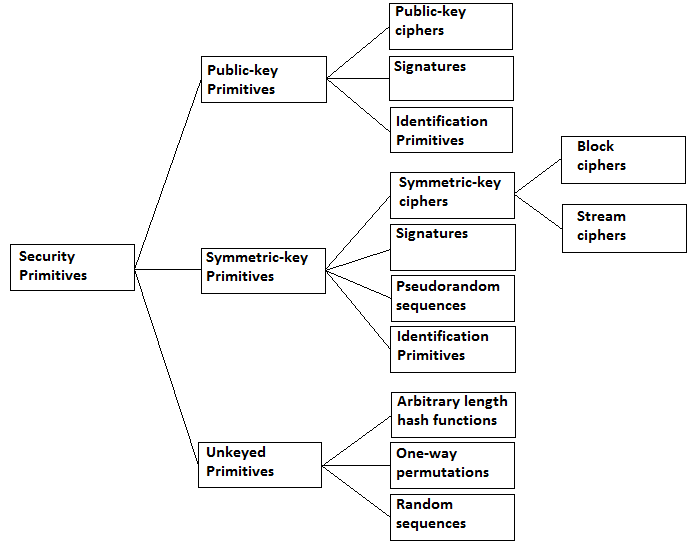
\includegraphics[width=0.82\textwidth]{securityPrimitives}
%	\caption{A taxonomy of cryptographic primitives}
%	\label{fig:secPrim}
%\end{figure}
%%info handbook strana 23

\subsection{Symmetric Cryptography}
%The beginnings of symmetric cryptography date back to around 2000 BC.\cite{singh2011code}. 
Symmetric encryption, as the name suggests, means that the encryption and decryption of 
plaintext are based on sharing a together secret - keys. The secret key could be a number, a 
word or just string of random letters. %This problem, however, stems directly from the provisions of a mystery. The problem of secure transfer of the message, in this case, is only converted to the issue of secure transmission of secret keys. This situation we can solve by other means, such as personal meetings or any infrastructure provided key distribution. Globally, all similar approaches proved to be unsuitable \cite{singh2011code}.
%\vskip 0.2in 

Symmetric ciphers could be divided into block and stream. Stream ciphers encrypt each character 
of plaintext separately, usually one bit. Block ciphers encrypt plaintext into blocks with 
fixed bit length \textit{n}. %Messages, which have more than \textit{n} bits, are separated into \textit{n}-bit blocks and then they are encrypted. 
%We distinguish several basic modes, such as ECB (Electronic Codebook), CBC (Cipher Block Chaining), CFB (Cipher Feedback) and OFB (Output Feedback), CTR (Counter Mode) \cite{piper2006kryptografie}.
%Stream ciphers are typically faster and easier for hardware implementation. They are often used in telecommunication applications, where we can use a very limited buffer. Their using is also advantageous in environment where is a significant probability of errors in the transmission because there is no propagation of this error to other data. In turn, block ciphers can perform the function Message Authentication Code (MAC) or hash functions.
%\vskip 0.2in 

The main disadvantage of symmetric cryptography is the necessity of a large number of keys 
and need of their distribution. For example, for together communication \textit{n} operators 
need to have \[ \frac{n * (n - 1)}{2}\] keys. It means that for the encrypted communications of 
midsize company with 50 employees, it would need to share 1225 different keys. 
%\vskip 0.2in

On the other hand, the advantage is the low computational complexity of symmetric ciphers. 
Their using is also useful in cases where the encrypted data are not sent anywhere, for example, 
to protect files on a personal computer.
 
\subsection{Asymmetric Cryptography}
%Unlike symmetric cryptography, asymmetric cryptography is very young. Its origins could be found in 1977 when the RSA cryptosystem was created based on the impossibility of effectively factorize of large numbers. In fact, the beginning of asymmetric cryptography was established a few years earlier by Clifford Cocks. His research, however, was still kept secret until recently \cite{singh2011code}.
%\vskip0.2in
Asymmetric cryptography allows data encryption and particularly the implementation of the 
digital signature. Each entity has two keys. The first is the private key that is used to 
decrypt a message or create a digital signature. It must be kept secret. The second key is 
public which is used for encryption and authentication of the digital signature. Of course, 
there is impossible to derive the private key from the public key.
%\vskip0.2in
%Asymmetric cryptography, itself, does not solve the authenticity of the public key. It is necessary to decide whether the given public key belongs to given entity. The solution of this problem is the infrastructure of the public key \cite{dostalek2016velky} which is nowadays the most widespread means of ensuring the credibility of the digital signature.
%\vskip0.2in

The main advantages of asymmetric cryptography are mainly a smaller number of keys than 
symmetric cryptography. If each entity has one public and one private key, it means that for 
\textit{n} entities are needed \textit{2n} keys. In the same situation as in the previous 
example, a company of 50 employees would need to ensure the safety of 100 keys, which is 
substantially less than 1225.
%\vskip0.2in

The biggest disadvantage of asymmetric cryptography is its slowness compared with symmetric 
cryptography. Therefore, they are most often used together, while the text is encrypted with a 
random symmetric encryption key. The key is encrypted using asymmetric ciphers. In the case of a 
digital signature, the first is created the fixed length hash of the message and then it is 
signed using asymmetric cryptography.

\subsection{Hash Function}
Hash functions are one of the basic elements of modern cryptography, often called one-way 
hash function.
%\vskip0.2in

Hash functions are effectively designed display binary strings unlimited length to binary 
strings a fixed length, called hash value. For a perfect hash function that has \textit{n}-bit 
hash value, there is a chance that a randomly selected string will be displayed on specific hash 
value $2^{-n}$. The basic idea of hash functions is that the hash value should serve as a 
representative of the input string. Hash function suitable for use in cryptography is usually 
chosen so that it is computationally very difficult find two different input strings that have 
the same hash value. If it succeeds in these two find strings, we say that we found a collision. 
Likewise, it should be computationally very difficult to find for a hash value corresponding to 
the input string. Using hash functions are used frequently to check the integrity of data and 
for digital signing of data \cite{piper2006kryptografie}.

ITEMIZE

\section{The X.509 Certificate}
Standard X.509 was originally designed as an authentication framework for X.500 
directories \cite{schmeh2006cryptography}. They have a hierarchical structure and the 
individual attributes can be assigned to individual computers of companies or individual 
printers. That is, each entity can be clearly identified, and each can have its private and 
public key. The proposal envisages the hierarchical structure of certificate authorities. 
Certificate X.509, see Figure \ref{fig:certificate}.
%\vskip0.2in
%The first version of the X.509 standard was already appeared in 1988 as the first proposal for PKI \cite{schmeh2006cryptography}. It was released by the International Telecommunication Union, Telecommunication Standardization Sector (ITU-T) cooperate with the International Organization for Standardization (ISO). It enabled its global adoption and extension. The first version was very simple and today is already inadequate. It contained only 7 fields:
%\vskip 0.2in
%\begin{itemize}[leftmargin=2em,rightmargin=1em,itemsep=0.75\parskip,parsep=0em,topsep=0em,partopsep=0em]
%\item certificate version;
%\item certificate series number;
%\item algorithm which signed certificate;
%\item name of certification authority which certificate released;
%\item identity of certificate owner;
%\item public key of certificate owner;
%\item certificate validity.
%\end{itemize}
%\vskip 0.2in
%The second version was introduced five years later in 1993 and brought only minimal changes \cite{schmeh2006cryptography}. It contained only two new fields:
%\vskip 0.2in
%\begin{itemize}[leftmargin=2em,rightmargin=1em,itemsep=0.75\parskip,parsep=0em,topsep=0em,partopsep=0em]
%\item unique identifier of the certificate owner;
%\item unique identifier of the certification authority.
%\end{itemize}
%\vskip 0.2in
%The second version did not solve the problems associated with the first version. Fields which was needed in this version, still missing \cite{schmeh2006cryptography}.
%\vskip0.2in
%The third version was introduced in 1996 and the full specification can be found in ITU-T Recommendation X.509 or under the name ISO/IEC 9594-8 \cite{X.509}. Its biggest and most important benefit is to support the expansion. It is defined a syntax that allows you to create custom certificate extension. It eliminates the major shortcomings of the two previous versions, but then appears some incompatibility. Each extension has a name and a field that is intended to indicate whether they are a critical or optional extension. Application, that can not work with extension marked as critical, must immediately reject this certificate. On the other hand, if the extension is optional, it can be ignored. To avoid uncontrolled growth expansion, in 1997 fourteen of them were fixed and became part of the standard \cite{schmeh2006cryptography}.

\begin{figure}[th]
	\centering
	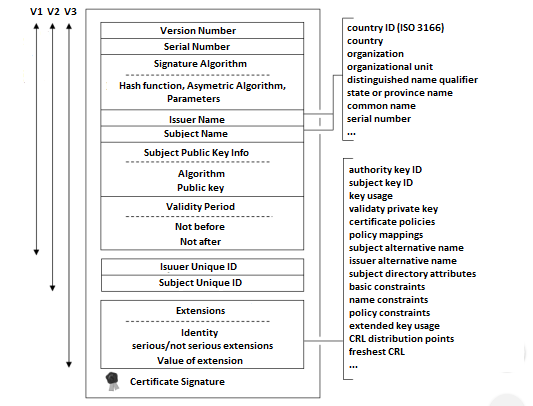
\includegraphics[width=1\textwidth]{certificate}
	\caption{Structure X.509 Certificate}
	\label{fig:certificate}
\end{figure}
%% Zdroj info o obrazku:
% @techreport{housley2002internet,
%   title={Internet X. 509 public key infrastructure certificate and % certificate revocation list (CRL) profile},
%   author={Housley, Russell and Polk, William and Ford, Warwick and Solo, David},
%  year={2002}
% }

To the protocols which mostly use X.509 certificates, belongs primarily SSL, TLS.

\section{Protocols SSL and TLS}
Protocols SSL and TLS are used for secure communications between client and server. They 
create a framework for the use of encryption and hash functions.
\vskip0.2in
SSL was developed by Netscape Communications which published three versions. The first version 
was only a test, the second has been used in practice. However, it still contained security 
vulnerabilities, the most important was susceptibility to attack \textit{man in the middle}. %zdroj?? https://scholar.google.sk/scholar?q=Security+Technologies+for+the+World+Wide+Web&btnG=&hl=sk&as_sdt=0%2C5 
The third version was introduced in 1996 and its specification could be found in the document \textit{The SSL Protocol Version 3.0} \cite{freier2011secure}. Of this version was created TLS protocol which is currently the most widespread and supported \cite{oppliger2003security}. There are three versions which have only minimal differences.
\vskip0.2in
Protocol SSL/TLS provides authentication of the two communicating parties by using asymmetric 
encryption, message integrity by using MAC and confidentiality by encrypting all communications 
by selected symmetric cipher.
\vskip0.2in
Protocol SSL/TLS is located between the application and the transport layer reference ISO/OSI 
model and consists of two main parts. They are \textit{The Record Layer Protocol} (RLP) and 
\textit{Handshake Protocol} (HP). %Part of HP are two auxiliary protocols - \textit{Change Cipher Specification Protocol} (CCSP) and \textit{Alert Protocol} (AP) \cite{oppliger2003security}.
\vskip0.2in
\textit{Record Layer Protocol} processes application data, performs fragmentation, compression 
and data encryption. On the other hand, it decrypts the data again and verifies the checksums. 
RLP protocol does not care about the type of encryption algorithm or encryption key setting. 
This information is from HP.

\textit{Handshake Protocol} is activated immediately after establishment the connection and 
provides identification of communicating parties, provision of cryptographic algorithms, 
compression algorithms and other attributes. Then it creates \textit{a master secret} from which 
are derived encryption keys, initiation vectors and the MAC. The process of the protocol is:
\vskip0.2in
\begin{enumerate}
\item The client wants to connect to the server and sends \textit{ClientHello}, which contains 
the highest number of version supported by SSL/TLS, the number of session (it is empty if it is 
a new session), the list of supported ciphers and compression methods and a random number.
\item The client waits for a response in the form of a report \textit{ServerHello}, which will 
contain the highest number of versions of SSL/TLS, which is supported by server and client. It 
will also contain encryption and compression method, which are selected from the list received 
in step one, a random number and its public key certificate (the server can also request 
authentication client).
\item The client verifies the server certificate, if all ciphers are satisfied. Next, he sends 
a request to server to exchange keys. At the end the server and client share a common 48 bits 
\textit{premaster secret}. \textit{The master secret} is derived from it. Then of the master 
secret and random numbers \textit{ClientHello ServerHello} are derived two session keys to 
encrypt messages and two MAC initiation vectors for use symmetric cipher in CBC mode. 
\item The client sends a confirmation selected ciphers. From this moment, the communication has 
been encrypted and the client sends a message that ends with this phase. In case the server 
required the client authentication, it has been carried out in this step. 
\item Finally, the server sends a confirmation used ciphers and message about the completion of 
this phase, thereby HP ends.
\end{enumerate}

%\textit{Change Cihper Specification Protocol} is a simple protocol that contains only a single message. It says there was the change of the encryption parameters and now only new ones will be used. It could be also called after the end of the initial phase.

%\textit{Alert protocol} provides the transmission of warning in case of any problem in communication - it contains an array of warning severity and description of the problem.
\vskip0.2in
The used algorithms:
\begin{itemize}[leftmargin=2em,rightmargin=1em,itemsep=0.75\parskip,parsep=0em,topsep=0em,partopsep=0em]
\item key exchange: RSA, Diffie-Hellman, ECDH;
\item stream symmetric ciphers: RC4 with key length of 40-120 bits;
\item block symmetric ciphers: DES, DES40, 3DES, IDEA;
\item hashing algorithms: MD5, SHA.
\end{itemize}
\vskip0.2in
TLS uses public key certificates for authentication. To establish a TLS connection are used 
symmetric keys (later called pre-shared keys or PSKs), shared in advance among the 
communicating parties \cite{eronen2005pre}.

\subsection{PSK Key Exchange Algorithm}

\chapter{Language GO}
Go is a programming language developed at \textit{Google} in year 2007 and announced in November 
2009. Many companies have started using Go because of its performance, simplicity, ease of use 
and powerful tooling. Go programming language is a statically-typed language with advanced 
features and a clean syntax \cite{doxsey2016introducing}. It combines the performance and 
security benefits associated with using a compiled language like \textit{C++} with the speed of 
a dynamic language like \textit{Python}. It provides:
\vskip0.2in
\begin{itemize}[leftmargin=2em,rightmargin=1em,itemsep=0.75\parskip,parsep=0em,topsep=0em,partopsep=0em]
\item garbage collector - memory is cleaned up automatically when nothing refers to it anymore,
\item fast compilation time - through effective work with addictions individual parts of the 
program and simple grammar,
\item light-weight processes (via goroutines), channels,
\item a rich standard library,
\item easy testing - incorporated directly into the core language,
\item one of the best documentation - a clear and full of examples.
\end{itemize}
\vskip0.2in

Go excluded some features intentionally to keep language simple and concise. There is no support 
for type inheritance, for method or operator overloading, for circular dependencies among 
packages, for pointer arithmetic, for assertions nor for generic programming.

\section{Packages}

\subsubsection{}

\begin{table}[th]
\begin{tabular}{|c c c|}
\hline
crypto & encoding & hash \\
\hline
aes & ascii85 & adler32 \\
cipher & asn1 & crc32 \\
des & base32 & crc64 \\
dsa & base64 & fnv \\
esdsa & biary &  \\
elliptic & csv &  \\
hmac & gob &  \\
md5 & hex &  \\
rand & json &  \\
rc4 & pem &  \\
rsa & xml &  \\
sha1 &  &  \\
sha356 &  &  \\
sha512 &  &  \\
subtle &  &  \\
tls &  &  \\
x509 \footnote{contains subpackage pkix} &  & \\ 
\hline
\end{tabular}
\caption{Table of cryptographic libraries created by golang} 
\label{table:crypto} 
\end{table}
% ZDROJ: https://golang.org/pkg/

\chapter{New chapter}

\begin{center}
\begin{longtable}[th]{|P{1.6cm}P{1cm}P{1cm}P{1cm}P{1.3cm}P{1.3cm}P{1.2cm}P{1.1cm}|}
\caption{Table of all cryptographic libraries in GO} \label{table:1} \\

\hline Name & Crypto. functions & Start of project & Is still opened & Issue tracker system & Doc. accessability & Number of downloads & License\\ \hline 
\endfirsthead

\multicolumn{8}{c}%
{{\tablename\ \thetable{} -- continued from previous page}} \\
\hline Name & Crypto. functions & Start of project & Is still opened & Issue tracker system & Doc. accessability & Number of downloads & License \\ \hline 
\endhead

\hline \multicolumn{8}{|r|}{{Continued on next page}} \\ \hline
\endfoot

\hline \hline
\endlastfoot

golang/ crypto & Y & 2009 & Y & Y & 5 &  & Y\\ 
%go-lang. cat-v.org/ pure-go-libs & N & \footnote{Page ceased updating in October, 2012} & & & & & Y \\ 
%golang libs.com category cryptography & Y & not all & 2012-2016 & some & & & \\
%golang libs.com category security & Y & not all & 2013-2016 & some & & & \\
ory-am/ fosite & asym, hash & 2015 & Y & Y & 4 & & Y \\
square/ go-jose & asym, sym & 2014 & Y & Y & 4 & & Y \\
Shopify/ ejson & hash & 2014 & Y & Y & 3 & & Y \\
mitchellh/ go-mruby & asym & 2014 & Y & Y & 4 & & Y \\
Sermo Digital/ jose & all & 2015 & Y & Y & 4 &  & Y \\
mozilla/ tls-observatory & hash & 2014 & Y & Y & 4 & & Y \\
square/ certigo & hash & 2016 & Y & Y & 3 & & Y \\
docker/ libtrust & all & 2014 & N & Y & 4 & & Y \\
dedis/ crypto & sym, hash & 2010 & Y & Y & 4 & & Y \\
dchest/ blake2b & hash & 2012 & N & Y & 4 & & Y \\
enceve/ crypto & hash & 2016 & N & Y & 4 & & Y \\
libp2p/ go-libp2p-crypto & all & 2015 & Y & Y & 4 &  & Y \\ 
dchest/ blake2s & hash & 2012 & N & N & 3 & & Y \\
benburkert/ openpgp & sym, hash & 2012 & N & N & 3 & & Y \\
minio/ sha256-simd & hash & 2016 & Y & Y & 3 & & Y \\
avelino/ awesome-go & un-known & 2014 & Y & Y & 4 & & Y \\
ethereum/ go-ethereum & all & 2013 & Y & Y & 4 & & Y \\
chain/ chain & hash & 2015 & Y & Y & 4 & & Y \\
lightning network/lnd & sym, hash & 2015 & Y & Y & 4 & & Y \\
square/ go-jose & asym, hash & 2014 & Y & Y & 4 & & Y \\
dgrijalva/ jwt-go & asym, hash & 2012 & Y & Y & 4 & & Y \\
golang/ oauth2 & asym, hash & 2014 & Y & Y & 4 & & Y  
\end{longtable}
\end{center}
%%  Zdroje k tabulke:
%%% https://golanglibs.com/top?q=security
%%% https://golanglibs.com/category/cryptography?sort=top
%%% http://go-lang.cat-v.org/pure-go-libs
%%% https://godoc.org/golang.org/x/crypto
%%% https://golang.org/pkg/
%%% ?


\printbibliography

\end{document}
